%=========================================================
\chapter{Modelo dinámico}	
\label{cap:modDinamico}

	Este capítulo se detallan todos los escenarios de ejecución del sistema. La figura~\ref{fig:CUcompleto1}  y la figurara~\ref{fig:CUcompleto2} muestra todos los casos de uso del sistema. En este documento solo detallamos los casos de uso del proyecto de gymnasios.

\begin{figure}[htbp]
	\begin{center}
		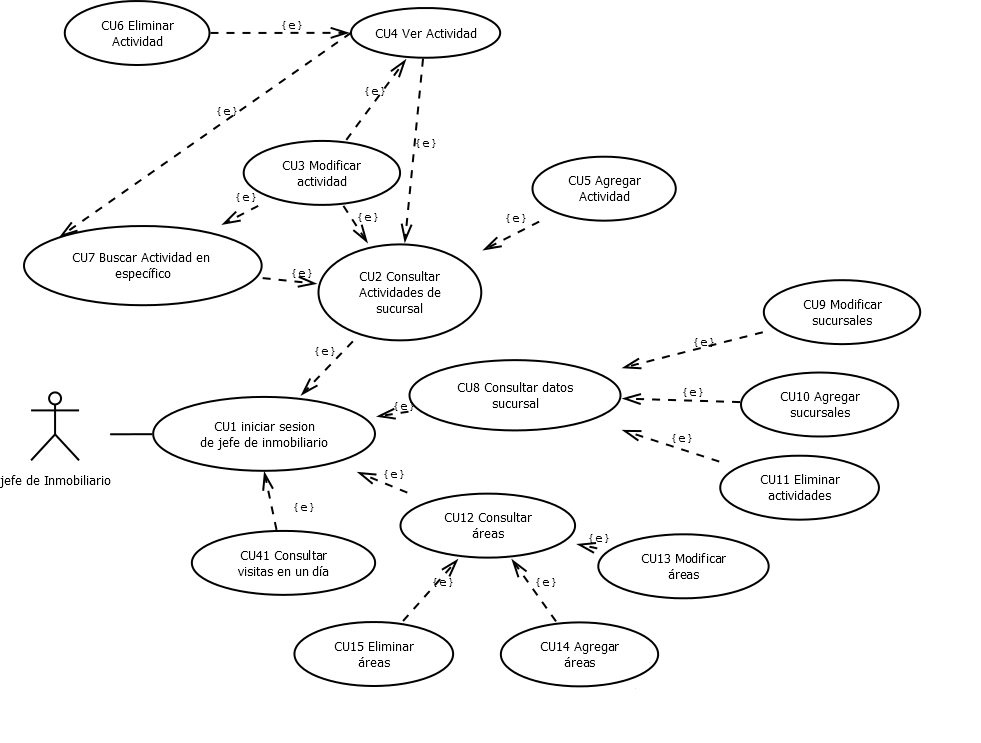
\includegraphics[angle=90, width=.7\textwidth]{images/CUcompleto1}
		\caption{Diagrama detallado del sistema parte 1.}
		\label{fig:CUcompleto1}
	\end{center}
\end{figure}

\begin{figure}[htbp]
	\begin{center}
		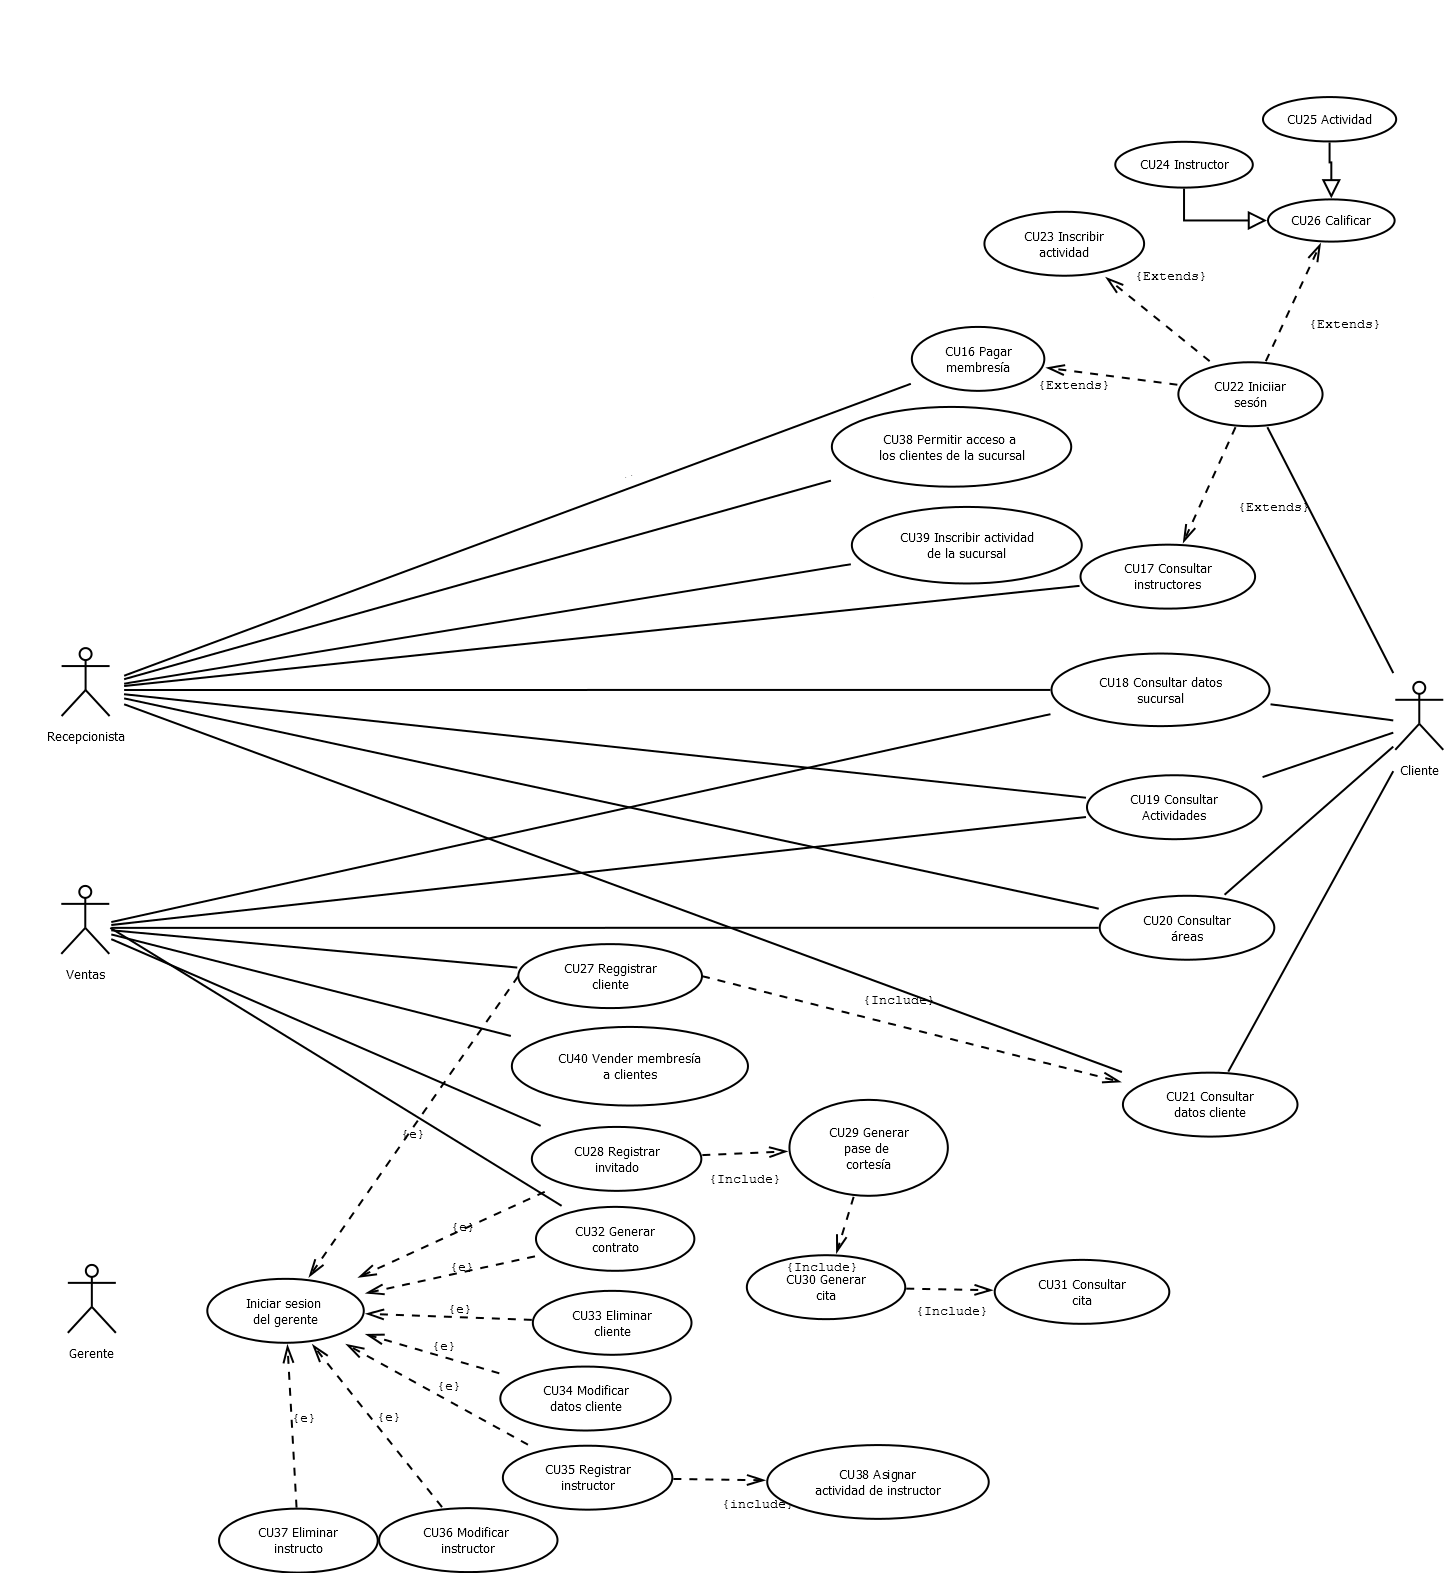
\includegraphics[angle=90, width=1.1\textwidth]{images/CUcompleto2}
		\caption{Diagrama detallado del sistema parte 1.}
		\label{fig:CUcompleto2}
	\end{center}
\end{figure}

%---------------------------------------------------------
\section{Descripción de actores}

%---------------------------------------------------------

A continuación se detallan los casos de uso.

%---------------------------------------------------------
% CASOS DE USO

% \IUref{IUAdmPS}{Administrar Planta de Selección}
% \IUref{IUModPS}{Modificar Planta de Selección}
% \IUref{IUEliPS}{Eliminar Planta de Selección}

% 


% Copie este bloque por cada caso de uso:
%-------------------------------------- COMIENZA descripción del caso de uso.

%\begin{UseCase}[archivo de imágen]{UCX}{Nombre del Caso de uso}{
%--------------------------------------
	\begin{UseCase}{CU1}{Iniciar sesión de jefe de inmobiliario}{
	
		Validar al jefe de inmobiliario para que pueda tener acceso a la información de la sucursal, modificar o eliminar datos a través del sistema.
	}
		\UCitem{Versión}{\color{Gray}0.4}
		\UCitem{Autor}{\color{Gray}Jazmin Camarillo Martínez}
		\UCitem{Supervisa}{\color{Gray}Francisco}
		\UCitem{Actor}{Jefe de inmobiliario}
		\UCitem{Propósito}{Para que el jefe de inmobiliario sea el único que pueda realizar acciones como eliminar modificar o agregar actividades, sucursales y áreas, y mantener la información actualizada.}
		\UCitem{Entradas}{Nombre de usurario y password.}
		\UCitem{Origen}{Teclado}
		\UCitem{Salidas}{mensaje de bienvenido, nombre completo del jefe de inmobiliario, cargo del J.I. nombre de la sucursal.}
		\UCitem{Destino}{Pantalla del jefe de inmobiliario.}
		\UCitem{Precondiciones}{El jefe de inmobiliario debe estar registrado, también debe tener una cuenta correcta para poder acceder como jefe de inmobiliario y que no haya una sesión iniciada.}
		\UCitem{Postcondiciones}{El jefe de inmobiliario deberá ver un menú con; perfil, sucursales, actividades y áreas, y sus datos de salida. }
		\UCitem{Errores}{}
		\UCitem{Tipo}{Caso de uso primario}
		\UCitem{Observaciones}{}
	\end{UseCase}
%--------------------------------------
	\begin{UCtrayectoria}{Principal}
		\UCpaso[\UCactor] Introduce su Nombre de usuario y su password para poder ingresar vía la  \IUref{IU1}{Pantalla de Inicio de Sesión del Jefe de Inmobiliario.}\label{CU1LoginJI}.
		\UCpaso[\UCactor] Confirma la operación presionando el botón Iniciar Sesión.
		\UCpaso Verifica que el nombre y password son correctos para ingresar sesión del jefe de inmobiliario.
		\UCpaso Despliega la \IUref{IU2}{Pantalla inicio del jefe de inmobiliario}.
	\end{UCtrayectoria}

%--------------------------------------		
		\begin{UCtrayectoriaA}{A}{El nombre de sesión no existe}
			\UCpaso[\UCactor] Muestra el Mensaje {\bf MSG1-}``El empleado [{\em Nombre de usuario}] no existe.''.
			\UCpaso[\UCactor] Introduce nombre usuario correcto.
			\UCpaso[] Continua con el paso 3 del \UCref{CU1}.
		\end{UCtrayectoriaA}
		
%--------------------------------------
		\begin{UCtrayectoriaA}{B}{Contraseña incorrecta}
			\UCpaso Muestra el Mensaje {\bf MSG1¿2-}``El password no es correcto.''.
			\UCpaso[\UCactor] Introduce password correcto.
			\UCpaso[] Continua con el paso 3 del \UCref{CU1}.
		\end{UCtrayectoriaA}


%--------------------------------------
% Puntos de extensión
\subsection{Puntos de extensión}
\UCExtenssionPoint{
	% Cuando:
	Desea acceder a las sucursales.
	Desea acceder a las actividades.
	Desea acceder a las áreas.
	Desea acceder a su perfil.
}{
	% Durante la región:
	En el paso 5.
}{
	% Casos de uso a los que extiende:
	\hyperlink{CU2}{CU2 Consultar Actividades de sucursal}.
}
		
		
% Copie este bloque por cada caso de uso:
%-------------------------------------- COMIENZA descripción del caso de uso.

%\begin{UseCase}[archivo de imágen]{UCX}{Nombre del Caso de uso}{
%--------------------------------------
\begin{UseCase}{CU2}{Consultar Actividades de sucursal}{
		Acceder al sistema a través del inicio de sesión del jefe de inmobiliario y ver datos generales de las actividades que hay en la sucursal.
	}
	\UCitem{Versión}{\color{Gray}0.4}
	\UCitem{Autor}{\color{Gray}Jazmin Camarillo Martínez}
	\UCitem{Supervisa}{\color{Gray}Francisco}
	\UCitem{Actor}{Jefe de inmobiliario}
	\UCitem{Propósito}{Para que el jefe pueda ver las actividades que tiene la sucursal y saber si sus datos son correctos y/o poderlos modificar.}
	\UCitem{Entradas}{Botón de actividad.}
	\UCitem{Origen}{Mouse}
	\UCitem{Salidas}{Nombre de la sucursal, nombre del isntructor, hora y dia dde la actividad.}
	\UCitem{Destino}{Pantalla del jefe de inmobiliario.}
	\UCitem{Precondiciones}{El jefe de inmobiliario debe inciiar sesion para ver las actividades, debe haber al menos una actividad.}
	\UCitem{Postcondiciones}{}
	\UCitem{Errores}{}
	\UCitem{Tipo}{Caso de uso primario}
	\UCitem{Observaciones}{}
\end{UseCase}
%--------------------------------------
\begin{UCtrayectoria}{Principal}
	\UCpaso[\UCactor] Introduce su Nombre de usuario y su password para poder ingresar vía la  \IUref{IU1}{Pantalla de Inicio de Sesión del Jefe de Inmobiliario.}\label{CU1LoginJI}.
	\UCpaso[\UCactor] Confirma la operación presionando el botón Iniciar Sesión.
	\UCpaso Verifica que el nombre y password son correctos para ingresar sesión del jefe de inmobiliario.
	\UCpaso Despliega la \IUref{IU2}{Pantalla inicio del jefe de inmobiliario}.
	\UCpaso[\UCactor] Selecciona en su menú el botón de las actividades. 
	\UCpaso Despliega la \IUref{IU3}{Pantalla Actividades}.
	
\end{UCtrayectoria}


%--------------------------------------
% Puntos de extensión
\subsection{Puntos de extensión}
\UCExtenssionPoint{
	% Cuando:
	Desee ver información completa de la actividad.
	Desee editar la información.
	Desee agregar una nueva actividad.
}{
	% Durante la región:
	En el paso 5.
}{
	% Casos de uso a los que extiende:
	\hyperlink{CU3}{CU3 Modificar actividad de sucursal}.
	\hyperlink{CU4}{CU4 Ver actividad de sucursal}.
	\hyperlink{CU5}{CU5 Agregar actividad de sucursal}.
	\hyperlink{CU6}{CU6 Buscar Actividad en específico}.
}		
		


%\begin{UseCase}[archivo de imágen]{UCX}{Nombre del Caso de uso}{
%--------------------------------------
\begin{UseCase}{CU3}{Modificar actividad de sucursal}{
	Modificar los datos permitidos a través de un formulario que despliega el sistema.
	}
	\UCitem{Versión}{\color{Gray}0.4}
	\UCitem{Autor}{\color{Gray}Jazmin Camarillo Martínez}
	\UCitem{Supervisa}{\color{Gray}Francisco}
	\UCitem{Actor}{Jefe de inmobiliario}
	\UCitem{Propósito}{Para que el jefe de inmobiliario pueda mantener la informacion correcta de las actividades que hay en el sistema.}
	\UCitem{Entradas}{Nombre de la actividad, el dia y la hora que se imparte la actividad, nombre del instructor,imagen(es) y descripcion.}
	\UCitem{Origen}{Mouse y teclado}
	\UCitem{Salidas}{Numero de actividad, nombre de la actividad, nombre de la sucursal, el dia y la hora que se imparte la actividad,nombre del instructor, la descripcion de la actividad, dirección de la sucursal, imagen(es) y mensaje de operación exitosa.}
	\UCitem{Destino}{Pantalla del jefe de inmobiliario.}
	\UCitem{Precondiciones}{La actividad debe estar registrada para poder ser modificada. Debe existir en el sistema el nombre del isntructor.}
	\UCitem{Postcondiciones}{La actividad quedará modificada con los nuevos datos, si es correcto el formato con el que se lleno el formulario, la información se verá actualizada en la consulta de ver actividad.}
	\UCitem{Errores}{Formulario no este llenado de acuerdo al formato.}
	\UCitem{Tipo}{Caso de uso primario}
	\UCitem{Observaciones}{Todos los campos del formulario son obligatorios.}
\end{UseCase}
%--------------------------------------
\begin{UCtrayectoria}{Principal}
	\UCpaso[\UCactor] Selecciona en su menú el botón de las actividades vía \IUref{IU3}{Pantalla Actividades}.
	\UCpaso Despliega la \IUref{IU3}{Pantalla Actividades}.
	\UCpaso[\UCactor] Selecciona botón de Editar que aparece en la \IUref{IU3}{Pantalla Actividades}.
	\UCpaso Despliega la \IUref{IU4}{Pantalla Editar Actividad}.
	\UCpaso[\UCactor] Selecciona el recuadro que quiera modificar .
	\UCpaso[\UCactor] Borra los datos del recuadro que seleccionó para poner el nuevo dato.
	\UCpaso[\UCactor] Pulsa el botón de aceptar para confirmar la operación que se realizó.
	\UCpaso Guarda los datos que están en los recuadros.	
	\UCpaso Despliega la \IUref{IU5}{Pantalla Edición terminada}.
	\UCpaso[\UCactor] Verifica que los datos estén como el desea y oprime el botón aceptar.
	\UCpaso Despliega la \IUref{IU3}{Pantalla Actividades}.
\end{UCtrayectoria}

%\BRref{BR129}{Determinar si un Estudiante puede inscribir Seminario.} \Trayref{A}
%--------------------------------------		
\begin{UCtrayectoriaA}{A}{El jefe de inmobiliario deja información en blanco}
	\UCpaso Muestra el Mensaje {\bf MSG3-}``Todos los campos son obligatorios.''.
	\UCpaso[\UCactor] Llena los campos faltantes.
	\UCpaso[\UCactor] Continua con el paso 8 del \UCref{CU3}.
\end{UCtrayectoriaA}


% Copie este bloque por cada caso de uso:
%-------------------------------------- COMIENZA descripción del caso de uso.

%\begin{UseCase}[archivo de imágen]{UCX}{Nombre del Caso de uso}{
%--------------------------------------
\begin{UseCase}{CU4}{Ver actividad de sucursal}{
		El sistema muestrará la información completa de una actividad seleccionada.
	}
	\UCitem{Versión}{\color{Gray}0.4}
	\UCitem{Autor}{\color{Gray}Jazmin Camarillo Martínez}
	\UCitem{Supervisa}{\color{Gray}Francisco}
	\UCitem{Actor}{Jefe de inmobiliario}
	\UCitem{Propósito}{Para que el jefe de inmobiliario pueda revisar que los datos de la actividad sean correctos.}
	\UCitem{Entradas}{botón de ver actividad.}
	\UCitem{Origen}{Teclado}
	\UCitem{Salidas}{Numero de actividad, nombre de la actividad, nombre de la sucursal, el dia y la hora que se imparte la actividad,nombre del instructor, la descripcion de la actividad, dirección de la sucursal, imagen(es).}
	\UCitem{Destino}{Pantalla del jefe de inmobiliario.}
	\UCitem{Precondiciones}{El jefe de inmobiliario debe estar dentro de susesión para poder ver la información. La actividad que desee ver, debe estar registrada.}
	\UCitem{Postcondiciones}{}
	\UCitem{Errores}{Actividad inexistente}
	\UCitem{Tipo}{Caso de uso primario}
	\UCitem{Observaciones}{}
\end{UseCase}
%--------------------------------------
\begin{UCtrayectoria}{Principal}
	\UCpaso[\UCactor] Ingresa a la \IUref{IU3}{Pantalla de Actividades.}\label{CU1LoginJI}.
	\UCpaso[\UCactor] Oprime el botón de ver.
	\UCpaso Despliega la \IUref{IU6}{Pantalla Ver Actividad}.
	\UCpaso Oprime el botón de aceptar para regresar a la  \IUref{IU3}{Pantalla de Actividades.}\label{CU1LoginJI}.
\end{UCtrayectoria}


%--------------------------------------
% Puntos de extensión
\subsection{Puntos de extensión}
\UCExtenssionPoint{
	% Cuando:
	Desea modificar datos de actividad.
}{
	% Durante la región:
	En el paso 3.
}{
	% Casos de uso a los que extiende:
	\hyperlink{CU3}{CU3 Modificar actividad de sucursal}.
}



% Copie este bloque por cada caso de uso:
%-------------------------------------- COMIENZA descripción del caso de uso.

%\begin{UseCase}[archivo de imágen]{UCX}{Nombre del Caso de uso}{
%--------------------------------------
\begin{UseCase}{CU5}{Agregar actividad a la sucursal}{
		El Jefe de inmobiliario podrá agregar una nueva actividad al sistema.
	}
	\UCitem{Versión}{\color{Gray}0.4}
	\UCitem{Autor}{\color{Gray}Jazmin Camarillo Martínez}
	\UCitem{Supervisa}{\color{Gray}Francisco}
	\UCitem{Actor}{Jefe de inmobiliario}
	\UCitem{Propósito}{Para que cada que se agregue una nueva actividad a la sucursal se pueda incorporar su información al sistema.}
	\UCitem{Entradas}{}
	\UCitem{Origen}{Teclado}
	\UCitem{Salidas}{.}
	\UCitem{Destino}{Pantalla del jefe de inmobiliario.}
	\UCitem{Precondiciones}{.}
	\UCitem{Postcondiciones}{El jefe de inmobiliario deberá ver un menú con; perfil, sucursales, actividades y áreas, y sus datos de salida. }
	\UCitem{Errores}{}
	\UCitem{Tipo}{Caso de uso primario}
	\UCitem{Observaciones}{}
\end{UseCase}
%--------------------------------------
\begin{UCtrayectoria}{Principal}
	\UCpaso[\UCactor] Introduce su Nombre de usuario y su password para poder ingresar vía la  \IUref{IU1}{Pantalla de Inicio de Sesión del Jefe de Inmobiliario.}\label{CU1LoginJI}.
	\UCpaso[\UCactor] Confirma la operación presionando el botón Iniciar Sesión.
	\UCpaso Verifica que el nombre y password son correctos para ingresar sesión del jefe de inmobiliario.
	\UCpaso Despliega la \IUref{IU2}{Pantalla inicio del jefe de inmobiliario}.
\end{UCtrayectoria}

%--------------------------------------		
\begin{UCtrayectoriaA}{A}{El nombre de sesión no existe}
	\UCpaso[\UCactor] Muestra el Mensaje {\bf MSG1-}``El empleado [{\em Nombre de sesión}] no existe.''.
	\UCpaso[\UCactor] Introduce nombre usuario correcto.
	\UCpaso[] Continua con el paso 3 del \UCref{CU1}.
\end{UCtrayectoriaA}

%--------------------------------------
\begin{UCtrayectoriaA}{B}{Contraseña incorrecta}
	\UCpaso Muestra el Mensaje {\bf MSG12-}``El password no es correcto.''.
	\UCpaso[\UCactor] Introduce password correcto.
	\UCpaso[] Continua con el paso 3 del \UCref{CU1}.
\end{UCtrayectoriaA}


%--------------------------------------
% Puntos de extensión
\subsection{Puntos de extensión}
\UCExtenssionPoint{
	% Cuando:
	Desea acceder a las sucursales.
	Desea acceder a las actividades.
	Desea acceder a las áreas.
	Desea acceder a su perfil.
}{
	% Durante la región:
	En el paso 5.
}{
	% Casos de uso a los que extiende:
	\hyperlink{CU2}{CU2 Consultar Actividades de sucursal}.
}

% \IUref{IUAdmPS}{Administrar Planta de Selección}
% \IUref{IUModPS}{Modificar Planta de Selección}
% \IUref{IUEliPS}{Eliminar Planta de Selección}

% 


% Copie este bloque por cada caso de uso:

%-------------------------------------- COMIENZA descripción del caso de uso.


%-------------------------------------- COMIENZA descripción del caso de uso.

%\begin{UseCase}[archivo de imágen]{CUX}{Nombre del Caso de uso}{
%--------------------------------------
	\begin{UseCase}{CU22}{Iniciar sesión cliente gimnasio}{
		Permite  al cliente del gimnasio autenticarse en el sistema mediante correo y su contraseña para poder ingresar a su cuenta.
	}
		\UCitem{Versión}{\color{Gray}0.2}
		\UCitem{Autor}{\color{Gray}Daniel.}
		\UCitem{Supervisa}{\color{Gray}Luis.}
		\UCitem{Actor}{\hyperlink{Cliente}{Cliente}}
		\UCitem{Propósito}{Que el cliente pueda pueda acceder a su información, actividades que tiene inscritas o para poder inscribir alguna y ver sus instructores.}
		\UCitem{Entradas}{Correo electrónico, contraseña}
		\UCitem{Origen}{El actor mediante el teclado ingresara los datos mencionados}
		\UCitem{Salidas}{Nombre completo, Dirección, Calle, No. int, No. Ext. Col. Del./Mun. C.P, Peso, Enfermedades, Alergias, Tipo de sangre, Medicamentos.}
		\UCitem{Destino}{Pantalla del cliente.}
		\UCitem{Precondiciones}{Que el cliente este registrado en el sistema, que no haya una sesión ya activa.}
		\UCitem{Postcondiciones}{El cliente va ver su pantalla de inicio.}
		\UCitem{Errores}{Que el correo sea incorrecto, que la contraseña sea errónea, que no este registrado.}
		\UCitem{Tipo}{Caso de uso primario}
		\UCitem{Observaciones}{Este caso de uso tendrá pestañas adicionales para ver sus actividades, horarios e instructores que tiene a demás de poder inscribir actividad. A grandes rasgos este C.U. solo muestra los datos personales del cliente del gimnasio.}
	\end{UseCase}
%--------------------------------------

	\begin{UCtrayectoria}{Principal}
		\UCpaso[\UCactor] Ingresa su correo.  %\IUref{IU23}{Pantalla de Control de Acceso}\label{CU17Login}.
		\UCpaso[\UCactor] Ingresa su contraseña.%\BRref{BR129}{Determinar si un Estudiante puede inscribir Seminario.} \Trayref{A}.
		\UCpaso[\UCactor] Da clic en el botón de iniciar sesión\Trayref{A}\label{CU15ValidarQR}.  %\IUref{IU32}{Pantalla de Selección de Seminario}
		\UCpaso valida que el usuario y contraseña son correctas para iniciar sesión. 
		\UCpaso mostrara el nombre completo, su direccion y los datos medicos..% \BRref{BR130}{Determinar si un Estudiante puede inscribirse en un Seminario} \Trayref{C}.
		\UCpaso  mostrara en el menu superior el nombre del usuario y una lista deplegable ahi mismo con la opción de ver cursos, ver instructores y cerrrar sesión.\Trayref{C}\label{CU15RealizarPago}. %\BRref{BR143}{Validar el horario del estudiante} \Trayref{D}.		
	\end{UCtrayectoria}

%--------------------------------------		


%--------------------------------------
% Puntos de extensión
%\subsection{Puntos de extensión}
%\UCExtenssionPoint{
	% Cuando:
%	Desea conocer las materias cursadas.
%}{
	% Durante la región:
%	Del paso 4 al paso 9.
%}{
	% Casos de uso a los que extiende:
%	\hyperlink{CU3.4}{CU3.4 Consultar historial académico}.
%}
		
		
		
%-------------------------------------- TERMINA descripción del caso de uso.


%-------------------------------------- COMIENZA descripción del caso de uso.

%\begin{UseCase}[archivo de imágen]{UCX}{Nombre del Caso de uso}{
%--------------------------------------
	\begin{UseCase}{CU23}{Inscribir actividad}{
		Permite  al cliente poder inscribirse en una actividad que se imparte en una sucursal.
	}
		\UCitem{Versión}{\color{Gray}0.1}
		\UCitem{Autor}{\color{Gray}Daniel}
		\UCitem{Supervisa}{\color{Gray}Luis}
		\UCitem{Actor}{\hyperlink{Cliente}{Cliente}}
		\UCitem{Propósito}{Que el usuario pueda ir a la actividad sin que le nieguen el acceso y conozca el horario en el que debe asistir.}
		\UCitem{Entradas}{Nombre Actividad, Sucursal, horario}
		\UCitem{Origen}{Teclado}
		\UCitem{Salidas}{Mensaje,Nombre Actividad,Sucursal,horario}
		\UCitem{Destino}{Pantalla del cliente}
		\UCitem{Precondiciones}{ Que el cliente haya iniciado sesión, que exista la actividades que se desea inscribir, que haya cupo en la actividad deseada.}
		\UCitem{Postcondiciones}{El cliente vera la actividad inscrita en su lista de actividades.}
		\UCitem{Errores}{No haya cupo en la actividad por inscribir}
		\UCitem{Observaciones}{}
	\end{UseCase}
%--------------------------------------
	\begin{UCtrayectoria}{Principal}
		\UCpaso[\UCactor] Desde la pantalla donde termina el CU22 seleccionar el botón de inscribir actividad.
		\UCpaso Muestra la pantalla de inscribir actividad.
		\UCpaso Muestra los campos que se deberán llenar para inscribir la actividad.
		\UCpaso[\UCactor] llena los campos y dar clic en inscribir.
		\UCpaso[\UCactor] confirma la operación oprimiendo el botón de aceptar. 
		\UCpaso Valida que la actividad y el horario que el usuario eligió exista.
		\UCpaso Valida que haya cupo en la actividad que eligió el usuario.
		\UCpaso Despliega msg3 "Actividad inscrita".
		\UCpaso Muestra la pantalla de inicio de cliente.	
	\end{UCtrayectoria}
%-------------------------------------- TERMINA descripción del caso de uso.


%-------------------------------------- COMIENZA descripción del caso de uso.

%\begin{UseCase}[archivo de imágen]{UCX}{Nombre del Caso de uso}{
%--------------------------------------
\begin{UseCase}{CU25}{Calificar Actividad.}{
		El cliente selecciona una puntuación para la actividad en un intervalo del 1 al 5 y se quedara guardada.
	}
	\UCitem{Versión}{\color{Gray}0.1}
	\UCitem{Autor}{\color{Gray}Daniel}
	\UCitem{Supervisa}{\color{Gray}Luis}
	\UCitem{Actor}{\hyperlink{Cliente}{Cliente}}
	\UCitem{Propósito}{ Que el cliente pueda transmitir una retro alimentación para el gimnasio y que pueda tener un mejor servicio. }
	\UCitem{Entradas}{Nombre Actividad, Calificación, Comentario }
	\UCitem{Origen}{Mouse y teclado.}
	\UCitem{Salidas}{Mensaje, Calificación}
	\UCitem{Destino}{Pantalla del cliente}
	\UCitem{Precondiciones}{ Que el cliente haya iniciado sesión, que este inscrito a alguna actividad.}
	\UCitem{Postcondiciones}{Que el cliente no este inscrito en la actividad que quiere calificar,que no exista la actividad que quiere calificar el cliente, que el cliente califique fuera del rango permitido.}
	\UCitem{Errores}{}
	\UCitem{Observaciones}{}
\end{UseCase}
%--------------------------------------

\begin{UCtrayectoria}{Principal}
	\UCpaso[\UCactor] Desde la pantalla donde termina el CU22 seleccionar el botón de Actividades.
	\UCpaso[\UCactor] Selecciona el botón de calificar actividad.
	\UCpaso Despliega los campos a llenar para calificar una actividad en la misma pantalla.
	\UCpaso[\UCactor] Selecciona una actividad
	\UCpaso[\UCactor] Asigna una calificación y un comentario que sera de manera opcional.
	\UCpaso[\UCactor] Confirma la operación oprimiendo el botón de "aceptar"..
	\UCpaso Valida que la actividad que seleccionó el usuario exista y que este inscrito en esa actividad.
	\UCpaso Mustra MSG4 "Calificación hecha" y la calificación de la actividad.
	
\end{UCtrayectoria}

<<<<<<< HEAD
%-------------------------------------- TERMINA descripción del caso de uso.

=======
<<<<<<< HEAD
%-------------------------------------- TERMINA descripción del caso de uso.
=======
e%-------------------------------------- TERMINA descripción del caso de uso.
>>>>>>> 0eff6495fec5e6e8df531b40918ac1ccee0f67e3
>>>>>>> 4435e9eea844c41d312547d202b75a2558a68b41



%\begin{figure}[htbp]
%	\begin{center}
%		\includegraphics[width=.8\textwidth]{images/vistas/buscarcliente}
%		\caption{Buscar cliente}
%		\label{fig:Ventas}
%	\end{center}
%\end{figure}

% \IUref{IUAdmPS}{Administrar Planta de Selección}
% \IUref{IUModPS}{Modificar Planta de Selección}
% \IUref{IUEliPS}{Eliminar Planta de Selección}

% 

%\begin{UseCase}[archivo de imágen]{UCX}{Nombre del Caso de uso}{
%--------------------------------------
\begin{UseCase}{CU34}{Registrar Instructor}{
		Crear un nuevo instructor en el sistema introduciendo sus datos personales y asignándole al menos una actividad.
	}
	\UCitem{Versión}{\color{Gray}0.4}
	\UCitem{Autor}{\color{Gray}Quiroz Olmedo Luis Eduardo}
	\UCitem{Supervisa}{\color{Gray}Francisco}
	\UCitem{Actor}{Gerente}
	\UCitem{Propósito}{Permitir al Gerente registrar nuevos Instructores en el sistema para que se les pueda asignar actividades nuevas o existentes y poder gestionar a los instructores.}
	\UCitem{Entradas}{•Nombre\newline
	•Dirección\newline
	•Nombre de Usuario\newline
	•Password}
	\UCitem{Origen}{Mouse y Teclado}
	\UCitem{Salidas}{Mensaje de confirmación.}
	\UCitem{Destino}{Pantalla de Instructores.}
	\UCitem{Precondiciones}{El jefe de inmobiliario debe inciiar sesion para ver las actividades, debe haber al menos una actividad.}
	\UCitem{Postcondiciones}{•Que el actor tenga una sesión iniciada
	\newline•Que el nombre de Usuario no este dado de alta en el sistema}
	\UCitem{Errores}{•Campos de Texto nulos o incompletos.\textbf{Trayectoria Alternativa A y B} \newline
	•Todas las actividades ocupadas.\textbf{Trayectoria Alternativa C}\newline
	•El actor no selecciona ninguna actividad.\textbf{Trayectoria Alternativa D}\newline}
	\UCitem{Tipo}{Caso de uso primario}
	\UCitem{Observaciones}{Todos los campos del formulario son obligatorios.}
\end{UseCase}
%--------------------------------------
\begin{UCtrayectoria}{Este caso de uso inicia cuando un actor se encuentra en la pantalla de \IUref{IU35}{Pantalla de Instructores}}
	\UCpaso[\UCactor] selecciona el boton ''Agregar Nuevo Instructor''.
	\UCpaso despliega la pantalla \IUref{IU351}{Pantalla Nuevo Instructor}
	\UCpaso[\UCactor]introduce el nombre completo del instructor en el campo de texto “Nombre completo”.
	\UCpaso sistema valida que los valores introducidos cumplen con las caracteristicas de un nombre.[aA-zA]
	\UCpaso[\UCactor]introduce la dirección del instructor en el campo de texto “Dirección”.
	\UCpaso sistema valida que los valores introducidos cumplen con las caracteristicas de una dirección.[aA-zA1-9 '.' '-']
	\UCpaso[\UCactor]introduce un nombre de usuario del instructor en el campo de texto “Nombre de Usuario”.
	\UCpaso sistema valida que los valores introducidos cumplen con las caracteristicas de un nombre [aA-zA0-9] y que el nombre de usuario no exista.
	\UCpaso[\UCactor]introduce un password del instructor en el campo de texto “Password”.
	\UCpaso sistema valida que los valores introducidos cumplen con las caracteristicas de una password.[aA-zA1-9]{8}
	\UCpaso selecciona el boton "Nueva Actividad"
	\UCpaso consulta que actividades tienen horarios libres y las despliega en la pantalla en forma de lista.
	\UCpaso[\UCactor] selecciona una actividad.
	\UCpaso \IUref {CU38}
	\UCpaso [\UCactor] da clic en el icono guardar.
	\UCpaso valida que al menos una actividad ha sido asignada.
	\UCpaso crea una nueva entidad Instructor con los datos introducidos ligado con las o la actividad seleccionadas y sus horarios seleccionados.
	\UCpaso despliega la pantalla \IUref{IU35}{Pantalla de Instructores} con el mensaje {\bf MSG7-} “Registro Exitoso”.
\end{UCtrayectoria}
%--------------------------------------
\begin{UCtrayectoriaA}{A}{El campo ''Nombre completo'' tiene menos de dos palabras o es nulo.}
			\UCpaso despliega un mensaje dentro del campo con la leyenda “Nombre invalido” y limpia el campo “Nombre Completo” y se continúa en el paso [1].
\end{UCtrayectoriaA}
%--------------------------------------
\begin{UCtrayectoriaA}{B}{El campo ''Direción'' tiene menos de dos palabras o es nulo.}
			\UCpaso despliega un mensaje dentro del campo con la leyenda “Dirección invalida” y limpia el campo “Direccion” y se continúa en el paso [1].
\end{UCtrayectoriaA}
%--------------------------------------
\begin{UCtrayectoriaA}{C}{Todas las Actividades se encuentran ocupadas}
		   \UCpaso despliega un mensaje en pantalla con la leyenda {\bf MSG8-} “No se cuenta con Actividades disponibles para asignar”.
		   \UCpaso despliega la pantalla \IUref{IU35}{Pantalla de Instructores} cancelando el registro y no guardando ningún dato.
\end{UCtrayectoriaA}
%--------------------------------------
\begin{UCtrayectoriaA}{D}{El actor no selecciono ninguna actividad}
		   \UCpaso despliega un mensaje en pantalla con la leyenda {\bf MSG9-} “Se debe seleccionar al menos una actividad” y se continua en el paso [9].	  
\end{UCtrayectoriaA}
%--------------------------------------
\begin{UCtrayectoriaA}{E}{El actor selecciona el boton ''Cancelar''}
		   \UCpaso muestra una alerta en pantalla con la leyenda {\bf MSG10-} “Estas seguro que deseas Cancelar” y dando las opciones Aceptar y Cancelar.
		   \UCpaso[\UCactor] selecciona ''Aceptar''.
		   \UCpaso despliega la pantalla \IUref{IU35}{Pantalla de Instructores}cancelando el registro y no guardando ningún dato.
\end{UCtrayectoriaA}

%--------------------------------------

%-------------------------------------- COMIENZA descripción del caso de uso.

%\begin{UseCase}[archivo de imágen]{UCX}{Nombre del Caso de uso}{
%--------------------------------------
\begin{UseCase}{CU35}{Listar Instructores}{
		El sistema genera una lista de todos los instructores que se encuentran activos.
	}
	\UCitem{Versión}{\color{Gray}0.4}
	\UCitem{Autor}{\color{Gray}Quiroz Olmedo Luis}
	\UCitem{Supervisa}{\color{Gray}Francisco}
	\UCitem{Actor}{Sistema}
	\UCitem{Propósito}{Listar solo los Instructores que no se encuentran declarados con bandera de borrado y mostrarlos para su edición.}
	\UCitem{Entradas}{}
	\UCitem{Origen}{}
	\UCitem{Salidas}{Lista de entidad Insctructor}
	\UCitem{Destino}{Pantalla de Instructores}
	\UCitem{Precondiciones}{• Que almenos exista un Instructor registrado}
	\UCitem{Postcondiciones}{Se tendrá la lista de todos los Instructores registrados}
	\UCitem{Errores}{•Todos los instructores se encuentran bloqueados o no hay instructores registrados.\textbf{Trayectoria Alternativa A}}
	\UCitem{Tipo}{Caso de uso secundario}
	\UCitem{Observaciones}{}
\end{UseCase}
%--------------------------------------
\begin{UCtrayectoria}{El caso de uso inicia cuando se va a desplegar la pantalla \IUref{IU35}{Instructores}}
	\UCpaso extrae todos los instructores que no cuentan con la bandera de borrado.
	\UCpaso genera una lista de instructores con los instructores del paso [1].
	\UCpaso muestra la pantalla  \IUref{IU35}{Instructores} con la lista del paso [2].
\end{UCtrayectoria}

%--------------------------------------		
\begin{UCtrayectoriaA}{A}{Todos los instructores se encuentran bloqueados o no hay instructores registrados}
	\UCpaso despliega en la pantalla \IUref{IU35}{Instructores} con el mensaje {\bf MSG13-} ''No hay instructores disponibles''.
\end{UCtrayectoriaA}

%--------------------------------------


% Copie este bloque por cada caso de uso:
%-------------------------------------- COMIENZA descripción del caso de uso.

%\begin{UseCase}[archivo de imágen]{UCX}{Nombre del Caso de uso}{
%--------------------------------------
	\begin{UseCase}{CU36}{Modificar Instructor}{
		Poder modificar los datos personales de un instructor y sus actividades asignadas.
	}
		\UCitem{Versión}{\color{Gray}0.4}
		\UCitem{Autor}{\color{Gray}Quiroz Olmedo Luis Eduardo}
		\UCitem{Supervisa}{\color{Gray}Francisco}
		\UCitem{Actor}{Gerente}
		\UCitem{Propósito}{Que los datos ingresados al momento de dar de alta un instructor puedan modificarse, así como también poder asignar nuevas actividades o editar las existentes asignadas a un instructor.}
		\UCitem{Entradas}{Instructor}
		\UCitem{Origen}{Teclado}
		\UCitem{Salidas}{Mensaje de confirmación}
		\UCitem{Destino}{Pantalla de Instructores.}
		\UCitem{Precondiciones}{ •Que el actor tenga una sesión iniciada en el sistema.\newline
        • Que el sistema tenga al menos un instructor y una actividad registrada.
}
		\UCitem{Postcondiciones}{El Instructor seleccionado ha sido modificado y se ve el cambio en la pantalla de Intructores}
		\UCitem{Errores}{
		 • El actor dejo los campos Nombre y Dirección completamente vacíos.\textbf{Trayectoria Alternativa B}\newline
		 El actor dejo el campo de “Actividades Asignadas” sin ninguna actividad.\textbf{Trayectoria Alternativa C}.
		}
		\UCitem{Tipo}{Caso de uso primario}
		\UCitem{Observaciones}{}
	\end{UseCase}
%--------------------------------------
	\begin{UCtrayectoria}{Este caso de uso inicia cuando un actor se encuentra en la pantalla \IUref{IU35}{Pantalla de Instructores} y tiene una sesión iniciada.}
		\UCpaso[\UCactor] selecciona el icono de edición sobre el instructor que se va a modificar.
		\UCpaso despliega la pantalla \IUref{IU352}{Pantalla Editar Instructor}
		\UCpaso permite editar los campos de texto “Nombre” y “Dirección”.
		\UCpaso[\UCactor] introduce un Nombre y Dirección nuevos.
		\UCpaso consulta las actividades con horarios libres y las despliega en la pantalla en forma de lista.
		\UCpaso[\UCactor] selecciona una actividad.
		\UCpaso consulta los horarios disponibles de la actividad seleccionada y los despliega en la pantalla en forma de lista.
		\UCpaso[\UCactor] selecciona un horario.
		\UCpaso[\UCactor] selecciona el boton guardar.
		\UCpaso actualiza los campos de nombre y dirección con los valores introducidos en el paso 4.
		\UCpaso \IUref {CU38}
		\UCpaso despliega la pantalla \IUref{IU352}{Instructores} con el mensaje {\bf MSG4-}``El Instructor [{\em Nombre de Instructor}] ha sido actualizado con éxito.''.
	\end{UCtrayectoria}

%--------------------------------------		
		\begin{UCtrayectoriaA}{A}{El actor NO introduce un nombre o dirección nuevos.}
			\UCpaso deja los campos “Nombre” y “Dirección” sin ningún cambio.
		\end{UCtrayectoriaA}
		
%--------------------------------------
		\begin{UCtrayectoriaA}{B}{El actor deja vacío el campo “Nombre” o “Dirección” o ambos campos.}
			\UCpaso despliega un mensaje dentro del campo con la leyenda {\bf MSG5-}``Campo Requerido'' .
		\end{UCtrayectoriaA}
%--------------------------------------
		\begin{UCtrayectoriaA}{C}{El actor NO selecciona ninguna actividad.}
			\UCpaso despliega un mensaje en pantalla con la leyenda {\bf MSG6-}``Asignar al menos una actividad'' .
		\end{UCtrayectoriaA}
%--------------------------------------
		\begin{UCtrayectoriaA}{D}{El actor selecciona el icono de borrado de la actividad }
			\UCpaso muestra una alerta en pantalla con el mensaje “Seguro que deseas eliminar la actividad” y las opciones “Aceptar” y “Cancelar”.
		    \UCpaso[\UCactor] selecciona la opción Aceptar.
		    \UCpaso elimina la relacion de con el horario y la actividad y la elimina de la lista de actividades asignadas.
		\end{UCtrayectoriaA}
%--------------------------------------
		\begin{UCtrayectoriaA}{E}{El actor selecciona la pestaña “Nueva Actividad”.}
			\UCpaso ejecuta los pasos [5-12].
		\end{UCtrayectoriaA}
%--------------------------------------
		\begin{UCtrayectoriaA}{F}{El sistema no tiene actividades disponibles}
			\UCpaso Muestra una alerta en pantalla con el mensaje "No hay actividades disponibles".
		\end{UCtrayectoriaA}		
%--------------------------------------
%\begin{UseCase}[archivo de imágen]{UCX}{Nombre del Caso de uso}{
%--------------------------------------
\begin{UseCase}{CU37}{Eliminar Instructor}{
		Eliminación de una entidad Instructor levantando una bandera de borrado sin eliminar los datos del Instructor.
	}
	\UCitem{Versión}{\color{Gray}0.4}
	\UCitem{Autor}{\color{Gray}Quiroz Olmedo Luis}
	\UCitem{Supervisa}{\color{Gray}Francisco}
	\UCitem{Actor}{Gerente}
	\UCitem{Propósito}{Evitar que se le asignen actividades al instructor que se desea borrar pero conservando sus datos personales.}
	\UCitem{Entradas}{Instructor}
	\UCitem{Origen}{Mouse}
	\UCitem{Salidas}{Mensaje de confirmación}
	\UCitem{Destino}{Pantalla de Instructores.}
	\UCitem{Precondiciones}{• El actor debe tener una sesión iniciada\newline
	• Debe exister al menos un instructor registrado}
	\UCitem{Postcondiciones}{El Instructor seleccionado ha sido eliminado.}
	\UCitem{Errores}{-}
	\UCitem{Tipo}{Caso de uso primario}
	\UCitem{Observaciones}{-}
\end{UseCase}
%--------------------------------------
\begin{UCtrayectoria}{Este caso de uso inicia cuando un actor se encuentra en la pantalla \IUref{IU352}{Pantalla Editar Instructor}}
	\UCpaso[\UCactor] selecciona el botón ''Eliminar'' en la columna del instructor que desea eliminar.
	\UCpaso despliega una alerta en pantalla {\bf ALERT5-} ''Seguro que deseas eliminar al instructor'' con las opciones ''Aceptar'' y ''Cancelar''.
	\UCpaso[\UCactor]selecciona la opción ''Aceptar''.
	\UCpaso levanta una bandera de borrado a la entidad del instructor seleccionado.
	\UCpaso desvincula los horarios de las actividades asiganadas al instructor borrado y las deja visibles para su posible asignación a otros instructores.
	\UCpaso borra al instructor de la lista de instructores en la pantalla \IUref{IU352}{Pantalla Editar Instructor}
	\UCpaso despliega la pantalla \IUref{IU352}{Pantalla Editar Instructor} con el mensaje {\bf MSG12-} ''Borrado Exitoso''.
\end{UCtrayectoria}
%--------------------------------------		
\begin{UCtrayectoriaA}{A}{El actor selecciona el botón “Cancelar”}

	\UCpaso despliega la pantalla \IUref{IU352}{Pantalla Editar Instructor} sin ejecutar ningún cambio.

\end{UCtrayectoriaA}


%--------------------------------------

% Copie este bloque por cada caso de uso:
%-------------------------------------- COMIENZA descripción del caso de uso.

%\begin{UseCase}[archivo de imágen]{UCX}{Nombre del Caso de uso}{
%--------------------------------------
\begin{UseCase}{CU38}{Asignar Actividad al Instructor}{
	Asignar una entidad Actividad seleccionada previamente con una entidad Instructor.
	}
	\UCitem{Versión}{\color{Gray}0.4}
	\UCitem{Autor}{\color{Gray}Quiroz Olmedo Luis}
	\UCitem{Supervisa}{\color{Gray}Francisco}
	\UCitem{Actor}{Gerente}
	\UCitem{Propósito}{Crear una unión con una actividad seleccionada y un horario y para evitar duplicados en asignaciones de actividades}
	\UCitem{Entradas}{Actividad}
	\UCitem{Origen}{Mouse y teclado}
	\UCitem{Salidas}{-}
	\UCitem{Destino}{Pantalla de Editar Instructor o Registrar Instructor}
	\UCitem{Precondiciones}{• Que el sistema tenga al menos un instructor y una actividad registrados.\newline
	• Que el actor haya seleccionado una actividad.
	}
	\UCitem{Postcondiciones}{Quedara unido un horario de la Actividad seleccionada con un Instructor.}
	\UCitem{Errores}{Formulario no este llenado de acuerdo al formato.}
	\UCitem{Tipo}{Caso de uso secundario}
	
\end{UseCase}
%--------------------------------------
\begin{UCtrayectoria}{Este caso de uso inicia cuando un actor se encuentra en la pantalla de \IUref{IU35}{Instructor} o en la pantalla \IUref{IU352}{Pantalla Editar Instructor}  y seleccionó una actividad disponible}
	\UCpaso consulta los horarios que no han sido asignados de la actividad seleccionada y los despliega en la pantalla en forma de lista.
	\UCpaso[\UCactor] selecciona el horario.
	\UCpaso el sistema elimina de la lista de horarios disponibles el horario seleccionado.
	\UCpaso el sistema reserva el horario para que ya no sea mostrado en alguna sesion existente.
	\UCpaso el sistema liga el horario seleccionado con el Instructor que se esta editando.
\end{UCtrayectoria}

%\BRref{BR129}{Determinar si un Estudiante puede inscribir Seminario.} \Trayref{A}
%--------------------------------------		
\begin{UCtrayectoriaA}{A}{No hay horarios disponibles de la actividad seleccionada.}
	\UCpaso muestra un mensaje en pantalla con la leyenda {\bf MSG11-} ''Sin horarios disponibles''.
	\UCpaso redirecciona ala pantalla \IUref{IU352}{Pantalla Editar Instructor} o  \IUref{IU35}{Instructor} dependiendo de donde venga la selección.
	%\UCpaso[\UCactor] Continua con el paso 8 del \UCref{CU3}.
\end{UCtrayectoriaA}
%--------------------------------------		
\begin{UCtrayectoriaA}{B}{El actor no selecciona ningún horario}

	\UCpaso muestra un mensaje en pantalla con la leyenda {\bf MSG12-} ''Se debe seleccionar al menos un horario'' y se continua en el paso [2].
\end{UCtrayectoriaA}


% Copie este bloque por cada caso de uso

%-------------------------------------- TERMINA descripción del caso de uso.


\begin{UseCase}{CU39}{Vender membresia a clientes}{
		El actor desde su pagina de inicio da clic al boton de vender membresia en la cual se le pide el correo al cliente y despues se selecciona la membresia que escoge el cliente y despues se genera el contrato para el cliente.}
	\UCitem{Versión}{\color{Gray}0.1}
	\UCitem{Autor}{\color{Gray}Daniel}
	\UCitem{Supervisa}{\color{Gray}Luis}
	\UCitem{Actor}{\hyperlink{Vendedor}{Vendedor}}
	\UCitem{Propósito}{ Que el cliente pueda tener acceso a las instalaciones y que se pueda realizar la venta con mas facilidad.}
	\UCitem{Entradas}{Correo del cliente,nombe del cliente,tipo de membresia.}
	\UCitem{Origen}{Mouse, teclado}
	\UCitem{Salidas}{Datos generales del cliente,Contrato de venta en pdf.}
	\UCitem{Destino}{Pantalla del actor,Impresora.}
	\UCitem{Precondiciones}{ Que el cliente no tenga una membresia del mimso tipo.}
	\UCitem{Postcondiciones}{Se registrara el cliente en el sistema.}
	\UCitem{Errores}{Que el cliente no este regisrado en el sistema.}
	\UCitem{Observaciones}{ninguna.}
\end{UseCase}
%--------------------------------------

\begin{UCtrayectoria}{Principal}
	\UCpaso[\UCactor] Accede la página de ventas de membresia.
	\UCpaso Despliega una pantalla con un campo para ingresar el correo y un boton para realizar la busqueda.
	\UCpaso[\UCactor] Ingresa el correo en el campo.  
	\UCpaso[\UCactor] presiona el botón de buscar.
	\UCpaso Valida que el correo este en el sistema.\Trayref{A}.
	\UCpaso Muestra una pantalla con los datos del cliente y los tipos de membresia que se tiene para poder seleccionar solo una de ellas.
	\UCpaso [\UCactor] Seleciona el tipo de membresia que pidio el cliente.
	\UCpaso Muestra un mensaje de confirmacion de la compra con dos botones: aceptar y cancelar.
	\UCpaso[\UCactor] Seleciona aceptar.\Trayref{B}
	\UCpaso añade en el sistema que el cliente tiene ya una membresia.
	\UCpaso Genera el contrato y lo manda a la impresora.
\end{UCtrayectoria}

%--------------------------------------		
		\begin{UCtrayectoriaA}{A}{El cliente no esta en registrado en el sistema.}
			\UCpaso Muestra mensaje que no esta registrado .
		\end{UCtrayectoriaA}
%--------------------------------------		
		\begin{UCtrayectoriaA}{B}{El cliente no accede a la venta.}
			\UCpaso[\UCactor] Selecciona el boton de cancelar.
			\UCpaso Muestra la pagina principal de venta donde se pide el correo del cliente.
		\end{UCtrayectoriaA}
		
%-------------------------------------- TERMINA descripción del caso de uso.

% Copie este bloque por cada caso de uso:



\section{Guión de Pruebas}

\subsection{Guión de prueba 1}
\begin{itemize}
\item ID: Guión 01
\item ALCANCE: CU01
\item NOMBRE: Iniciar sesioón de jefe de inmobiliario  
\item PREPARACIÓN:\\
-En la BD debe de estar registrado el jefe de inmobiliario.
\item CP 1:
\item DATOS DE ENTRADA:\\
	\begin{itemize}
		\item Correo electrónico del J.I: Jefe\_inmobiliario\@hotmail.com
		\item Contraseña: SOY\_elJefe1
	\end{itemize}
\begin{center}			
	\begin{tabular}{|l|l|l|l|}
		\hline
		CP 1\\
		PASOS\\
		\hline 1.- Ingresar a la pantalla IU08\\
		\hline 2.- Introducir el numero de cliente.\\
		\hline 3.- Presionar el botón buscar\\
		\hline
	\end{tabular}
\end{center}
\item SALIDAS: Verificación y resultado si tiene acceso permitido el usuario a las diferentes 
áreas del gimnasio.
\item CP 2:
\item DATOS DE ENTRADA:\\
-numero de empleado: 354\\
\begin{center}			
	\begin{tabular}{|l|l|l|l|}
		\hline
		CP 2\\
		PASOS\\
		\hline 1.- Ingresar a la pantalla IU08\\
		\hline 2.- Introducir el numero de cliente.\\
		\hline 3.- Presionar el botón buscar\\
		\hline
	\end{tabular}
\end{center}
\item SALIDAS: Verificación y resultado si tiene acceso permitido el usuario a las diferentes 
\item CP 3:
\item DATOS DE ENTRADA:\\
-numero de cliente: -123\\
\begin{center}			
	\begin{tabular}{|l|l|l|l|}
		\hline
		CP 3\\
		PASOS\\
		\hline 1.- Ingresar a la pantalla IU08\\
		\hline 2.- Introducir el numero de cliente.\\
		\hline 3.- Presionar el botón buscar\\
		\hline
	\end{tabular}
\end{center}
\item SALIDAS: "Sin especificar".
\item CP 4:
\item DATOS DE ENTRADA:\\
-numero de cliente: 500\\
\begin{center}			
	\begin{tabular}{|l|l|l|l|}
		\hline
		CP 4\\
		PASOS\\
		\hline 1.- Ingresar a la pantalla IU08\\
		\hline 2.- Introducir el numero de cliente.\\
		\hline 3.- Presionar el botón buscar\\
		\hline
	\end{tabular}
\end{center}
\item SALIDAS: Muestra una pantalla con un formulario de datos a llenar del cliente.
\end{itemize}

<<<<<<< HEAD
% \IUref{IUAdmPS}{Administrar Planta de Selección}
% \IUref{IUModPS}{Modificar Planta de Selección}
% \IUref{IUEliPS}{Eliminar Planta de Selección}

% 

%\begin{UseCase}[archivo de imágen]{UCX}{Nombre del Caso de uso}{
%--------------------------------------

\begin{itemize}
\item \textbf{ID}: CP 35
\item \textbf{ALCANCE}: CU35
\item \textbf{NOMBRE}: Registrar Instructor
\item \textbf{PREPARACIÓN}:\\
		-El Gerente tiene que tener una sesión iniciada.
		-Debe existir al menos una Actividad Registradaen la DB.
\begin{itemize}
\item \textbf{CP 1}:
\item \textbf{DATOS DE ENTRADA}:\\
-Luis Quiroz\\
-Record 56, Col. portales,CDMX.\\
-LuisQ\\
-12345678\\
	\begin{center}			
	\begin{tabular}{||l|l|l|l||}
		\hline
		\hline
			CP 1\\
			PASOS\\
			\hline 1.- Se selecciona el boton ''Agregar Instructor''\\
			\hline 2.- Se instroduce ''Luis Quiroz'' en el campo  Nombre Completo.\\
			\hline 3.- Se instroduce ''Record 56, Col. portales,CDMX.'' en el campo  Dirección.\\
			\hline 4-. Se introduce  ''LuisQ'' en el campo Nombre de Usuario.\\
			\hline 5-. Se introduce  12345678  en el campo Password.\\
            \hline 6.-Se da clic en el botón ''Nueva Actividad''\\
            \hline 7-.Se selecciona la actividad ''Pesas''\\
            \hline 8.-Se da clic en el botón ''Guardar''.\\
        \hline
		\hline
	\end{tabular}
	\end{center}
\item \textbf{SALIDAS}: Redirección a la pantalla \IUref{IU3}{Editar Instructor} y aparece la leyenda \textbf{Registro Exitoso}.
\end{itemize}
\begin{itemize}
\item \textbf{CP 2}:
\item \textbf{DATOS DE ENTRADA}:\\
-LuisQU\\
-12345678\\
	\begin{center}			
	\begin{tabular}{||l|l|l|l||}
		\hline
		\hline
			CP 2\\
			PASOS\\
			\hline 1.- Se selecciona el boton ''Agregar Instructor''\\
			\hline 4-. Se introduce  ''LuisQU'' en el campo Nombre de Usuario.\\
			\hline 5-. Se introduce  12345678  en el campo Password.\\
            \hline 6.-Se da clic en el botón ''Nueva Actividad''\\
            \hline 7-.Se selecciona la actividad ''Pesas''\\
            \hline 8.-Se da clic en el botón ''Guardar''.\\
        \hline
		\hline
	\end{tabular}
	\end{center}
\item \textbf{SALIDAS}:Aparece en el campo 'Nombre Completo' la leyenda \textbf{Nombre Invalido} y en el campo 'Dirección' la leyenda \textbf{Dirección Invalida} .
\end{itemize}
\end{itemize}
%------------------------------------------------------

\begin{itemize}
\item \textbf{ID}: CP 36
\item \textbf{ALCANCE}: CU 36
\item \textbf{NOMBRE}: Modificar Instructor
\item \textbf{PREPARACIÓN}:\\
		-El Gerente tiene que tener una sesión iniciada.
		-Debe existir al menos una Actividad Registrada en la DB.
		-Debe existir al menos un Instructor Registrada en la DB.
\begin{itemize}
\item \textbf{CP 1}:
\item \textbf{DATOS DE ENTRADA}:\\
-Selección Instructor "Daniel Romero"
-Daniel Romero Lopez
	\begin{center}			
	\begin{tabular}{||l|l|l|l||}
		\hline
		\hline
			CP 1\\
			PASOS\\
			\hline 1.- Se selecciona el boton de edición\\
			\hline 2.- Se despliega la pantalla con los datos del instructror.\\
			\hline 3.- Se introduce en el campo de nombre la cadena ''Daniel Romero Lopez''.\\
			\hline 4-. Se selecciona la actividad ''Pesas''\\
			\hline 5-. Se selecciona el horario '''8:00-9:00''\\
            \hline 6.-Se da clic en el botón ''Guardar''\\
        \hline
		\hline
	\end{tabular}
	\end{center}
\item \textbf{SALIDAS}: Redirección a la pantalla \IUref{IU3}{Instructor} y aparece la leyenda ''Daniel Romero Lopez ha actualizado con éxito''
\end{itemize}
\begin{itemize}
\item \textbf{CP 2}:
\item \textbf{DATOS DE ENTRADA}:\\
-Selección Instructor "Daniel Romero"
-Daniel Romero Lopez
	\begin{center}			
	\begin{tabular}{||l|l|l|l||}
		\hline
		\hline
			CP 2\\
			PASOS\\
			\hline 1.- Se selecciona el boton de edición\\
			\hline 2.- Se despliega la pantalla con los datos del instructror.\\
			\hline 3.- Se introduce en el campo de nombre la cadena ''Daniel Romero Lopez''.\\
			\hline 4-. Se borra el campo 'Dirección'\\
			\hline 4-. Se selecciona la actividad ''Pesas''\\
			\hline 5-. Se selecciona el horario '''8:00-9:00''\\
            \hline 6.-Se da clic en el botón ''Guardar''\\
        \hline
		\hline
	\end{tabular}
	\end{center}
\item \textbf{SALIDAS}:Aparece en el campo 'Dirección' la leyenda \textbf{Campo Requerido}.
\end{itemize}
\end{itemize}
%------------------------------------------------------

\begin{itemize}
\item \textbf{ID}: CP 37
\item \textbf{ALCANCE}: CU 37
\item \textbf{NOMBRE}: Eliminar Instructor
\item \textbf{PREPARACIÓN}:\\
		-El Gerente tiene que tener una sesión iniciada.\\
		-Debe existir al menos un Instructor Registrada en la DB.
\begin{itemize}
\item \textbf{CP 1}:
\item \textbf{DATOS DE ENTRADA}:\\
-Selección Instructor "Daniel Romero"
	\begin{center}			
	\begin{tabular}{||l|l|l|l||}
		\hline
		\hline
			CP 1\\
			PASOS\\
			\hline 1.- Se selecciona el boton de ''eliminar''\\
			\hline 2.- Se despliega una alerta con la leyenda ''seguro que deas eliminar al instructor''\\ y las opciones ''Aceptar'' y ''Cancelar''.\\
			\hline 3.- Se selcciona la opción ''Aceptar''\\
        \hline
		\hline
	\end{tabular}
	\end{center}
\item \textbf{SALIDAS}: Redirección a la pantalla \IUref{IU3}{Instructor} y aparece la leyenda ''Borrado exitoso'' y ya no se aprecia en la tabla al instructor borrado.
\end{itemize}
\begin{itemize}
\item \textbf{CP 2}:
\item \textbf{DATOS DE ENTRADA}:\\
-Selección Instructor "Daniel Romero"
	\begin{center}			
	\begin{tabular}{||l|l|l|l||}
		\hline
		\hline
			CP 2\\
			PASOS\\
			\hline 1.- Se selecciona el boton de ''eliminar''\\
			\hline 2.- Se despliega una alerta con la leyenda ''seguro que deas eliminar al instructor'\\' y las opciones ''Aceptar'' y ''Cancelar''.\\
			\hline 3.- Se selcciona la opción ''Cancelar''\\
        \hline
		\hline
	\end{tabular}
	\end{center}
\item \textbf{SALIDAS}:Se muestra la pantalla \IUref{IU3}{Instructor} sin  ningún cambio.
\end{itemize}
\end{itemize}
%------------------------------------------------------

\begin{itemize}
\item \textbf{ID}: CP 38
\item \textbf{ALCANCE}: CU 38
\item \textbf{NOMBRE}: Asignar Actividad al Instructor
\item \textbf{PREPARACIÓN}:\\
		-El Gerente tiene que tener una sesión iniciada.\\
		-Debe existir al menos un Instructor Registrada en la DB.
		-Debe existir al menos una Acttividad Registrada en la DB.
		-Se debe haber seleccionado una Actividad.
\begin{itemize}
\item \textbf{CP 1}:
\item \textbf{DATOS DE ENTRADA}:\\
	\begin{center}			
	\begin{tabular}{||l|l|l|l||}
		\hline
		\hline
			CP 1\\
			PASOS\\
			\hline 1.- Se Despliegan los horarios disponibles\\
			\hline 2.- Se selecciona el horario 8:00-9:00\\
        \hline
		\hline
	\end{tabular}
	\end{center}
\item \textbf{SALIDAS}: Se aprecia en la pantalla que se asigno el horario seleccionado.
\end{itemize}
\begin{itemize}
\item \textbf{CP 2}:
\item \textbf{DATOS DE ENTRADA}:\\
-Selección Instructor "Daniel Romero"
	\begin{center}			
	\begin{tabular}{||l|l|l|l||}
		\hline
		\hline
			CP 2\\
			PASOS\\
			\hline 1.- Se Despliegan los horarios disponibles\\
        \hline
		\hline
	\end{tabular}
	\end{center}
\item \textbf{SALIDAS}:Se muestra la pantalla \IUref{IU3}{Instructor} la leyenda \textbf{Se debe seleccionar al menos un horario}.
\end{itemize}
\end{itemize}
%------------------------------------------------------

=======
% \IUref{IUAdmPS}{Administrar Planta de Selección}
% \IUref{IUModPS}{Modificar Planta de Selección}
% \IUref{IUEliPS}{Eliminar Planta de Selección}

% 

%\begin{UseCase}[archivo de imágen]{UCX}{Nombre del Caso de uso}{
%--------------------------------------

\begin{itemize}
\item \textbf{ID}: CP 35
\item \textbf{ALCANCE}: CU35
\item \textbf{NOMBRE}: Registrar Instructor
\item \textbf{PREPARACIÓN}:\\
		-El Gerente tiene que tener una sesión iniciada.
		-Debe existir al menos una Actividad Registradaen la DB.
\begin{itemize}
\item \textbf{CP 1}:
\item \textbf{DATOS DE ENTRADA}:\\
-Luis Quiroz\\
-Record 56, Col. portales,CDMX.\\
-LuisQ\\
-12345678\\
	\begin{center}			
	\begin{tabular}{||l|l|l|l||}
		\hline
		\hline
			CP 1\\
			PASOS\\
			\hline 1.- Se selecciona el boton ''Agregar Instructor''\\
			\hline 2.- Se instroduce ''Luis Quiroz'' en el campo  Nombre Completo.\\
			\hline 3.- Se instroduce ''Record 56, Col. portales,CDMX.'' en el campo  Dirección.\\
			\hline 4-. Se introduce  ''LuisQ'' en el campo Nombre de Usuario.\\
			\hline 5-. Se introduce  12345678  en el campo Password.\\
            \hline 6.-Se da clic en el botón ''Nueva Actividad''\\
            \hline 7-.Se selecciona la actividad ''Pesas''\\
            \hline 8.-Se da clic en el botón ''Guardar''.\\
        \hline
		\hline
	\end{tabular}
	\end{center}
\item \textbf{SALIDAS}: Redirección a la pantalla \IUref{IU3}{Editar Instructor} y aparece la leyenda \textbf{Registro Exitoso}.
\end{itemize}
\begin{itemize}
\item \textbf{CP 2}:
\item \textbf{DATOS DE ENTRADA}:\\
-LuisQU\\
-12345678\\
	\begin{center}			
	\begin{tabular}{||l|l|l|l||}
		\hline
		\hline
			CP 2\\
			PASOS\\
			\hline 1.- Se selecciona el boton ''Agregar Instructor''\\
			\hline 4-. Se introduce  ''LuisQU'' en el campo Nombre de Usuario.\\
			\hline 5-. Se introduce  12345678  en el campo Password.\\
            \hline 6.-Se da clic en el botón ''Nueva Actividad''\\
            \hline 7-.Se selecciona la actividad ''Pesas''\\
            \hline 8.-Se da clic en el botón ''Guardar''.\\
        \hline
		\hline
	\end{tabular}
	\end{center}
\item \textbf{SALIDAS}:Aparece en el campo 'Nombre Completo' la leyenda \textbf{Nombre Invalido} y en el campo 'Dirección' la leyenda \textbf{Dirección Invalida} .
\end{itemize}
\end{itemize}
%------------------------------------------------------

\begin{itemize}
\item \textbf{ID}: CP 36
\item \textbf{ALCANCE}: CU 36
\item \textbf{NOMBRE}: Modificar Instructor
\item \textbf{PREPARACIÓN}:\\
		-El Gerente tiene que tener una sesión iniciada.
		-Debe existir al menos una Actividad Registrada en la DB.
		-Debe existir al menos un Instructor Registrada en la DB.
\begin{itemize}
\item \textbf{CP 1}:
\item \textbf{DATOS DE ENTRADA}:\\
-Selección Instructor "Daniel Romero"
-Daniel Romero Lopez
	\begin{center}			
	\begin{tabular}{||l|l|l|l||}
		\hline
		\hline
			CP 1\\
			PASOS\\
			\hline 1.- Se selecciona el boton de edición\\
			\hline 2.- Se despliega la pantalla con los datos del instructror.\\
			\hline 3.- Se introduce en el campo de nombre la cadena ''Daniel Romero Lopez''.\\
			\hline 4-. Se selecciona la actividad ''Pesas''\\
			\hline 5-. Se selecciona el horario '''8:00-9:00''\\
            \hline 6.-Se da clic en el botón ''Guardar''\\
        \hline
		\hline
	\end{tabular}
	\end{center}
\item \textbf{SALIDAS}: Redirección a la pantalla \IUref{IU3}{Instructor} y aparece la leyenda ''Daniel Romero Lopez ha actualizado con éxito''
\end{itemize}
\begin{itemize}
\item \textbf{CP 2}:
\item \textbf{DATOS DE ENTRADA}:\\
-Selección Instructor "Daniel Romero"
-Daniel Romero Lopez
	\begin{center}			
	\begin{tabular}{||l|l|l|l||}
		\hline
		\hline
			CP 2\\
			PASOS\\
			\hline 1.- Se selecciona el boton de edición\\
			\hline 2.- Se despliega la pantalla con los datos del instructror.\\
			\hline 3.- Se introduce en el campo de nombre la cadena ''Daniel Romero Lopez''.\\
			\hline 4-. Se borra el campo 'Dirección'\\
			\hline 4-. Se selecciona la actividad ''Pesas''\\
			\hline 5-. Se selecciona el horario '''8:00-9:00''\\
            \hline 6.-Se da clic en el botón ''Guardar''\\
        \hline
		\hline
	\end{tabular}
	\end{center}
\item \textbf{SALIDAS}:Aparece en el campo 'Dirección' la leyenda \textbf{Campo Requerido}.
\end{itemize}
\end{itemize}
%------------------------------------------------------

\begin{itemize}
\item \textbf{ID}: CP 37
\item \textbf{ALCANCE}: CU 37
\item \textbf{NOMBRE}: Eliminar Instructor
\item \textbf{PREPARACIÓN}:\\
		-El Gerente tiene que tener una sesión iniciada.\\
		-Debe existir al menos un Instructor Registrada en la DB.
\begin{itemize}
\item \textbf{CP 1}:
\item \textbf{DATOS DE ENTRADA}:\\
-Selección Instructor "Daniel Romero"
	\begin{center}			
	\begin{tabular}{||l|l|l|l||}
		\hline
		\hline
			CP 1\\
			PASOS\\
			\hline 1.- Se selecciona el boton de ''eliminar''\\
			\hline 2.- Se despliega una alerta con la leyenda ''seguro que deas eliminar al instructor''\\ y las opciones ''Aceptar'' y ''Cancelar''.\\
			\hline 3.- Se selcciona la opción ''Aceptar''\\
        \hline
		\hline
	\end{tabular}
	\end{center}
\item \textbf{SALIDAS}: Redirección a la pantalla \IUref{IU3}{Instructor} y aparece la leyenda ''Borrado exitoso'' y ya no se aprecia en la tabla al instructor borrado.
\end{itemize}
\begin{itemize}
\item \textbf{CP 2}:
\item \textbf{DATOS DE ENTRADA}:\\
-Selección Instructor "Daniel Romero"
	\begin{center}			
	\begin{tabular}{||l|l|l|l||}
		\hline
		\hline
			CP 2\\
			PASOS\\
			\hline 1.- Se selecciona el boton de ''eliminar''\\
			\hline 2.- Se despliega una alerta con la leyenda ''seguro que deas eliminar al instructor'\\' y las opciones ''Aceptar'' y ''Cancelar''.\\
			\hline 3.- Se selcciona la opción ''Cancelar''\\
        \hline
		\hline
	\end{tabular}
	\end{center}
\item \textbf{SALIDAS}:Se muestra la pantalla \IUref{IU3}{Instructor} sin  ningún cambio.
\end{itemize}
\end{itemize}
%------------------------------------------------------

\begin{itemize}
\item \textbf{ID}: CP 38
\item \textbf{ALCANCE}: CU 38
\item \textbf{NOMBRE}: Asignar Actividad al Instructor
\item \textbf{PREPARACIÓN}:\\
		-El Gerente tiene que tener una sesión iniciada.\\
		-Debe existir al menos un Instructor Registrada en la DB.
		-Debe existir al menos una Acttividad Registrada en la DB.
		-Se debe haber seleccionado una Actividad.
\begin{itemize}
\item \textbf{CP 1}:
\item \textbf{DATOS DE ENTRADA}:\\
	\begin{center}			
	\begin{tabular}{||l|l|l|l||}
		\hline
		\hline
			CP 1\\
			PASOS\\
			\hline 1.- Se Despliegan los horarios disponibles\\
			\hline 2.- Se selecciona el horario 8:00-9:00\\
        \hline
		\hline
	\end{tabular}
	\end{center}
\item \textbf{SALIDAS}: Se aprecia en la pantalla que se asigno el horario seleccionado.
\end{itemize}
\begin{itemize}
\item \textbf{CP 2}:
\item \textbf{DATOS DE ENTRADA}:\\
-Selección Instructor "Daniel Romero"
	\begin{center}			
	\begin{tabular}{||l|l|l|l||}
		\hline
		\hline
			CP 2\\
			PASOS\\
			\hline 1.- Se Despliegan los horarios disponibles\\
        \hline
		\hline
	\end{tabular}
	\end{center}
\item \textbf{SALIDAS}:Se muestra la pantalla \IUref{IU3}{Instructor} la leyenda \textbf{Se debe seleccionar al menos un horario}.
\end{itemize}
\end{itemize}
%------------------------------------------------------

>>>>>>> 4435e9eea844c41d312547d202b75a2558a68b41

%---------------------------------------------------------
% PANTALLAS DE LOS CASOS DE USO
\IUfig[.5]{LoginJI}{IU1}{Pantalla de login del jefe de inmobiliario.}

\IUfig[.5]{InicioSesion}{IU2}{Pantalla de Inicio de Sesión del jefe de inmobiliario.}

\IUfig[.5]{ActividadesJI}{IU3}{Pantalla de Actividades.}

\IUfig[.5]{EditarActividad}{IU4}{Pantalla de Editar Actividad.}

\IUfig[.5]{FinEditarAC}{IU5}{Pantalla de Edición terminada.}

\IUfig[.5]{VerActividadJI}{IU6}{Pantalla de Ver Actividad.}





\IUfig[.5]{Instructores}{IU35}{Pantalla de Instructores.}

\IUfig[.5]{NuevoInstructor}{IU351}{Pantalla Nuevo Instructor.}

\IUfig[.5]{EditarInstructor}{IU352}{Pantalla Editar Instructor.}

\IUfig[.5]{loginCliente}{IU22}{Pantalla de Inicio de sesion del cliente.}

\IUfig[.5]{inicioCliente}{IU23}{Pantalla de Inicio del cliente.}



